\section{Gaussian Process regression}\label{GPR}

We adopted the GPy package \citep{gpy2014}, which is a Gaussian Process (GP) framework developed by the Sheffield machine learning group, to train GP models for the \textsc{MESA} Grid. 

\subsection{Gaussian process model}

GP models can be applied as probabilistic models to regression problems.  Here we will use the GP model to generalise a grid of stellar models to a continuous and probabilistic function that maps inputs (i.e., initial mass, composition, age, ...) to observable quantities (i.e., effective temperature, radius, $\Delta \nu$, ... ).  We aim to use the GP model as a non-parametric emulator, that is emulating the comparatively slow calls to models of stellar evolution. 

\subsubsection{Gaussian process application}

We start with a grid of stellar models containing $N$ models with a label we  want to learn, for example model effective temperature, which we will denote with the general symbol $\bf y$, and a set of input labels $\bf X$ (e.g., mass, age, and metallicity).  We can use a GP to make predictions of the effective temperature (or $y$) for additional input values given by $\bf X_{\star}$.  The vector $\bf y$ is arranged ${\bf y} = \left(y_{i}, ... ,y_{N} \right)^{T}$ where the subscript label references the stellar model.  The input labels are arranged into a $N \times D$ matrix where $D$ is the number of input dimensions (e.g., $D=3$ for mass, age, and metallicity) so that ${\bf X} = ({\bf x}_{1}, ..., {\bf x}_{N})^{T}$ where ${\bf x_{i}} = (x_{1, i}, ..., x_{D, i})^{T}$.  The matrix of additional inputs $\bf X_{\star}$ has the same form as $\bf X$ but size $N_{\star} \times D$.

Rasmussen and Williams (!REF!), from which our description below is based, define a GP as a collection of random variables, where any finite number of which have a joint Gaussian distribution.  In general terms, GP's may be written as
\begin{equation}
y({\bf x}) \sim \mathcal{GP}\left( m({\bf x}), {\bf \Sigma}\right),
\end{equation}
where $m({\bf x})$ is some mean function, and ${\bf \Sigma}$ is some covariance matrix.  The mean function controls the deterministic part of the regression and the covariance controls the stochastic part.  The mean function defined here could be any deterministic function and we will label the additional parameters, or hyperparameters, $\phi$.  Each element of the covariance matrix is defined by the covariance function or {\it kernel function} $k$ which has hyperparameters $\theta$ and is given by,
\begin{equation}
{\bf \Sigma}_{n, m} = k({\bf x}_{n}, {\bf x}_{m}),
\end{equation}
where the inputs ${\bf x}_{i}$ are $D$-dimensional vectors and the output is a scalar covariance.

As a GP is a collection of random variables, where any finite number of which have a joint Gaussian distribution, the joint probability of our data $\bf y$ is
\begin{equation}
p({\bf y} | {\bf X, \phi, \theta}) = \mathcal{N}(m({\bf X}), {\bf \Sigma}).
\end{equation}
If we want to obtain predictive distributions for the output $\bf y_{\star}$ given the inputs $\bf X_{\star}$ the joint probability distribution of $\bf y$ and $\bf y_{\star}$ is Gaussian and given by
\begin{equation}
p \left( \begin{bmatrix} {\bf y} \\ {\bf y_{\star}} \end{bmatrix} \right) = \mathcal{N} \left( \begin{bmatrix} {\bf X} \\ {\bf X_{\star}} \end{bmatrix} , \begin{bmatrix} {\bf \Sigma} & {\bf K_{\star} }\\ {\bf K_{\star}}^{T} & {\bf K_{\star \star}} \end{bmatrix}  \right), 
\end{equation}
where the covariance matrices $\bf \Sigma$ and $\bf K$ are computed using the kernel function so that
\begin{equation}
{\bf \Sigma}_{n, m} = k({\bf X}_{n}, \, {\bf X}_{m}),
\end{equation}
which is an $N \times N$ matrix.
\begin{equation}
{\bf K}_{\star \, n, m} = k({\bf X}_{n}, \, { \bf X}_{\star \, m}),
\end{equation}
which is an $N \times N_{\star}$ matrix, and finally
\begin{equation}
{\bf K}_{\star \star \, n, m} = k({\bf X}_{\star \, n},  {\bf X}_{\star \,m}),
\end{equation}
which is an $N_{\star} \times N_{\star}$ matrix.
The predictions of $\bf y_{\star}$ are again a Gaussian distribution so that,
\begin{equation}
{\bf y}_{\star} \sim \mathcal{N}(\bf \hat{y}_{\star}, \, \bf C),
\label{eq:pred}
\end{equation}
where 
\begin{equation}
{\bf \hat{y}}_{\star} = m({\bf X}_{\star}) + {\bf K}_{\star}^{T} \, {\bf \Sigma}^{-1} \, ({\bf y} - m(\bf X)),
\end{equation}
and 
\begin{equation}
{\bf C} = {\bf K}_{\star \star} - {\bf K}_{\star}^{T} \, {\bf \Sigma}^{-1} \, {\bf K_{\star}}.
\end{equation}

At point we can make predictions on model properties given a grid of stellar models using equation \ref{eq:pred}.  But these predictions will be poor unless we select sensible values for the form and hyperparameters of the mean function and covariance function.  In the following section we detail a number of kernel functions that will be tested against the data.  We will then discuss the method for determining the values of the hyperparameters to be used.

\subsubsection{GPR kernels}
The analysing is mainly based on the MLP kernel because of the following points (ask Guy to write some words about the MLP kernel).
We also use other couple kernels to improve the GPR model, particularly for the residuals of the MLP-kernel model.  
The kernels involved in this works are listed below:

\begin{itemize}
\item MLP: Multi Layer Perceptron kernel (also known as arc sine kernel or neural network kernel)
\item RBF: Radial Basis Function kernel (also known as squared exponential kernel)
\item RQ: Rational Quadratic Kernel (equivalent to adding together many RBF kernels with different lengthscales)
\item EXP: Exponential Kernel
\item Mat32: Matern 3/2 kernel
\end{itemize}

\subsubsection{Gaussian process likelihood function}

TODO

\subsection{GPR Model Inputs}
We aim to derive stellar parameters based on fundamental inputs of the model grid. As mentioned in Section~\ref{sec:grid}, our model grid has five independent fundamental inputs, says, mass, initial metallicity, initial helium fraction, mixing-length parameter, and the age.
GPR model inputs are ideally in fixed dynamic ranges (form a cube-like space), however, the age ranges significantly vary with the mass. We hence defined an age index as an input instead of the age. The age index is calculated on each evolutionary track following 
\begin{equation}
 \tau' = 10^{(\tau/\tau_{\rm max})},
\end{equation}
where $\tau$ is the age, $\tau_{\rm max}$ is the maximum age of an evolutaionary track. Note that $\tau_{\rm max}$ must be defined in the same way for all evolutionary tracks. In this work, we defined $\tau_{\rm max}$ as the age when a track evolves to $\log g$ = 3.6. The purpose to use an exponential formula is flattening sharp changes of global parameters around the 'hook' and the turn-off point. This makes GPR models converge easily. A comparison between GPR models using $\tau/\tau_{\rm max}$ and $10^{(\tau/\tau_{\rm max})}$ is illustrated in Figure~\ref{fig:selection_of_t}.  As it can be seen that, the effective temperature evolution presents a hump around 0.7 of the total lifetime (the hook) and quickly drops in the last 10\% lifetime. Using the age index instead of fractional age significantly smoothes the curve and make it easer to fit. We used the same kernel (MLP) and optimiser to fit both curves and compared residuals in the bottom panel. As it can be seen that, the GPR model using the age index showes better agreement with the original data especially for the hump ($\sim$6100K).

We summary our selections of GPR model inputs and outputs as below. 
\begin{itemize}
\item GPR model inputs and their dynamic ranges:
\item[] Mass ($M$ = 0.8 -- 1.2$M_{\odot}$)
\item[] Age index ($\tau'$ = 0.0 -- 10)
\item[] Initial metallicity ([Z/X]$_{\rm init}$ =  0.0015 -- 0.0572)
\item[] Initial helium fraction ($Y_{\rm init}$ = 0.24 -- 0.32)
\item[] Mixing-length parameter ($\alpha_{\rm MLT}$ = 1.7 -- 2.5)
\item GPR model outputs: 
\item[] Effective temperature ($T_{\rm eff}$) 
\item[] Surface gravity ($\log g$)
\item[] Radius ($R$)
\item[] Two global seismic parameters ($\Delta\nu$ and $\nu_{\rm max}$)  
\item[] Surface metallicity ([Z/X]$_{\rm surf}$)
\item[] Age ($\tau$)
\end{itemize}
Thus, our GPR model can be described as 
\begin{equation}\label{gprmodel}
{\rm Outputs} = f(M, t', ({\rm Fe/H})_{\rm init}, Y_{\rm init}, \alpha_{\rm MLT}). 
\end{equation}

\begin{figure}
	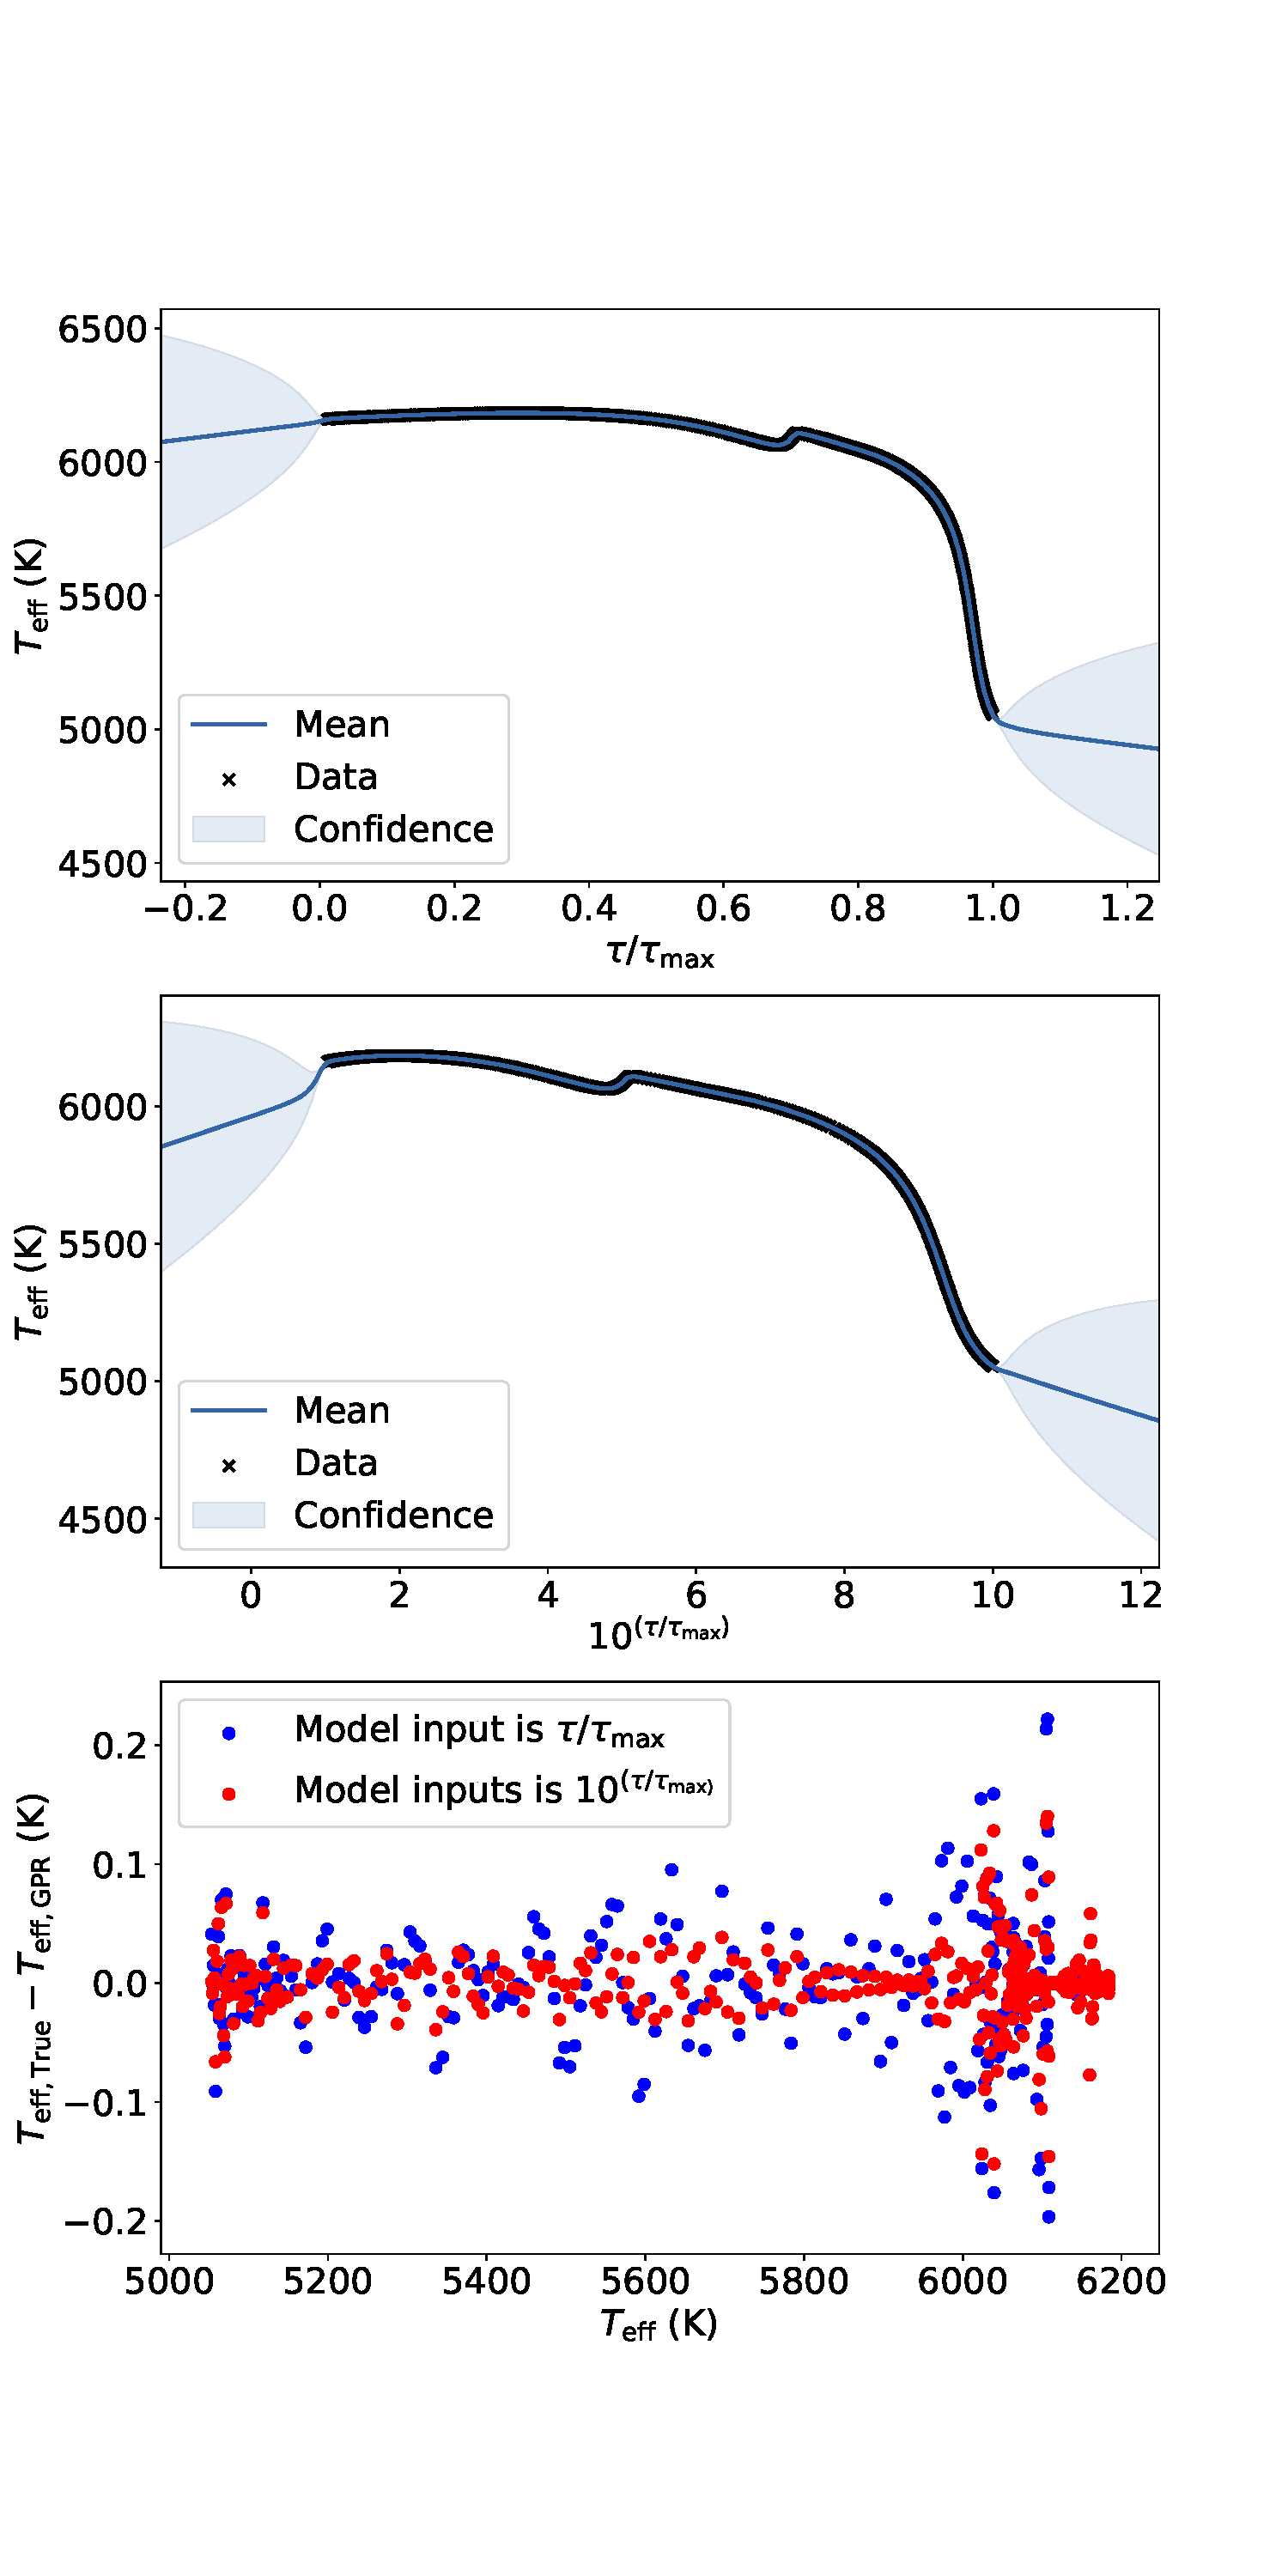
\includegraphics[width=1.0\columnwidth]{selection_of_t.pdf}
    \caption{The comparison between GPR model predictions with two different input age indices ($\tau/\tau_{\rm max}$ and $10^{(\tau/\tau_{\rm max})}$) for a 1.1$M_{\odot}$ track. Top: the GPR model of the effective temperature as a function of $\tau/\tau_{\rm max}$. The adopted kernel is MLP. Middle: same as the top, but the GPR model input is $10^{(\tau/\tau_{\rm max})}$). Bottom: residuals between true values and GPR model predictions. }
    \label{fig:selection_of_t}
\end{figure}
 

\subsection{Training Procdure}\label{workflow}
To demonstrate our work flow, we present our training process of a 2-demissions GPR model. The GPR model contents two inputs, namely, $M$ and $\tau'$,  and one output ($T_{\rm eff}$). We only adopted the stellar models with fixed [Fe/H]$_{\rm init}$ (0.0 dex), $Y_{\rm init}$ (0.28), and $\alpha_{\rm MLT}$ (2.1) from the primary grid. The total number of stellar models is 24,485. A validation data set was computed with the same model inputs but random masses. Our training procedure contents three major steps: data selection, model training, and model validation.      

\subsubsection{Step1: Data Selection}

As discussed in Section~\ref{grid}, we have three types of data for training, testing, and validating GPR models. The training data is apparently the model grid used to train GPR models.  The test dataset, which was also selected from the model grid but not used in any training processes. Test data are used to examine wether a GPR model gives proper description for the model grid. Once a GPR model provides good agreement with the testing data, the training succeeds. The last type is validation data, which are the off-grid models with random input parameters. Validation data are used to validate GPR models and also to estimate their systematical uncertainty. 

Because the computational and memory complexity exponentially increase with the number of data involved in the Gaussian Process. A practical limit of the training data is about 10,000. The testing and validation data could be massive but we set a limit of 50,000 for the efficiency.  This is to say, only a small subset of the model grid can be used. The sampling method is hence critical. The training data should uniformly cover the output ranges to avoid data gaps but also highly weight where quick changes occurs. %In our GPR model outputs, the five global parameters ($T_{\rm eff}$, $\log g$, $R$, $\delta \nu$, and $\nu_{\rm max}$) are tightly correlated during the evolution. They hence can be trained with the same data.
 Due to the \textsc{MESA} step-control strategy, stellar models are dense at the main-sequence and the red-giant phases but quite sparse on subgiant stage. Random sampling is hence not appropriate. We tested a few methods and found that using the displacement of each evolving step on the HR diagram as the weight gave the best sampling. The displacement is defined as $\delta d$ = $(\delta T_{\rm eff}^{2}$ + $\delta L^{2})^{1/2}$, where $\delta T_{\rm eff}$ and $\delta L^{2}$ are the differences between two consecutive models on the evolutionary track. We sampled on each evolutionary track separately and then combined the models as datasets. The sampling method gave a relatively uniform data distribution on the HR diagram and also highly weighted the regions around the hook and turn-off point.   
%
 %The data for the other two GPR outputs ($t$ and [Fe/H]$_{\rm surf}$) need to be separately sampled because of the evolutionary features.  
%
%The age mainly changes during main-sequence and slowly increases afterward. For this reason, we used the change of fractional age ($\delta t/t_{\rm max}$) at each step as the weight . The sampled data for training the age are hence much denser at the main-sequence than the evolved stages. 
% 
%The surface metallicity of an evolutionary track gradually reduces during main-sequence because of the element diffusion, however, rapidly increases at post main-sequence due to the quick expansion of the convective envelope. The training data ought to present evolving details at the giant phase and also properly cover that at the main-sequence. For this reason, we adopted the gradient of $(Z/X)_{\rm surf}$ as a function of the age index ($t'$) as the weight. We summarised the weight for a data point ($w_{i}$) on an evolutionary track as below:
%\begin{equation}\label{weights}
%w_{i} = \left\{\begin{matrix}
%\begin{aligned} 
 %& (\delta T_{\rm eff, i}^{2} + \delta L_{i}^{2})^{1/2} \; {\rm for}\;T_{\rm eff}, \log g, R, \delta \nu, {\rm and} \; \nu_{\rm max}, \\ 
%& \delta (Z/X)_{\rm surf, i}/\delta t' \;  {\rm for}\;(Z/X)_{\rm surf},\\ 
%& \delta \tau_{i}/\tau_{\rm max} \;  {\rm for}\;\tau.\\
%\end{aligned} 
%\end{matrix}\right.
%\end{equation}
%
%The test and validation data should uniformly cover the HR diagram for sensible statistical results. We hence used the sampling method for the five global parameters in Equation~\ref{weights} for these two types of data. 
%
We demonstrated our selection for data to train the 2-demission GPR model ($T_{\rm eff}$ = $f(M, t')$) in Figure~\ref{fig:data_on_hrd}.  Here we sampled 3,000 and 5,000 on-grid models as the training and test data, and 5,000 off-grid models as validation data.  

\begin{figure}
	\includegraphics[width=1.0\columnwidth]{2D_data_on_HR.pdf}
    \caption{Selected training and testing data for the GPR model with 2-demission inputs on the $T_{\rm eff}$ - $\log g$. Black, blue, and red dots represent training, test, and validation data. }
    \label{fig:data_on_hrd}
\end{figure}

\subsubsection{Step 2:  Model Training}

In the model training step, we applied a data-residual process, which is described as follow. 
A GPR model (M0 here after) is primarily trained with the training data and tested with the test data. If residuals of test data are significant large or present any local structures, an extra GPR model (M1 hereafter) will be trained to describe the first-order residuals. With M0 + M1, the second-order residual could be calculated and used to train another extra GPR model (M2 hereafter). The training process goes to $n$-order residuals (M$n$) until GPR predictions do not significantly improve. Thus, the process provides a series of GPR models as a combination to describe stellar evolutions. Here we illustrated the details the process by training the 2-demission GPR model ($T_{\rm eff}$ = $f(M, t')$). 

We firstly train the primary GPR model (M0) with the training dataset shown in Figure~\ref{fig:data_on_hrd}. We used the MLP kernel and optimise M0 with random initial hyperparameters. The result of M0 is demonstrated in Figure~\ref{fig:gpmodel}. It can be seen that the GPR model has transferred the model grid into a continued function (indicated by contour lines). For models below $\sim$1.05$M_{\odot}$, the $T_{\rm eff}$ contour lines are smooth and the GPR model give good description for the data. However, the structure becomes complex at $t'\sim5$ when $M$ is larger than 1.05 because of the appearance of the 'hook' in stellar evolution. And the GPR model predictions does not very convinced in this area. This can be seen in the left bottom panel in Figure~\ref{fig:drprocess}, which shows the offsets between M0 predictions and the test data (testing errors hereafter). The large offset in the local area indicate M0 does not well describe the whole grid. This is because we only used a small subset for training and did not pass enough details for the GPR model to learn. It is a common issue with the Gaussian process when training big data set because of the limitation of the size of training data. To mange this issue, we developed the data-residual process aiming to use multiple GPR models to describe the grid. This process is illustrated in Figure ~\ref{fig:drprocess}. After training and testing M0, we trained an extra GPR model (M1) to describe the 1st-order residuals. We randomly selected 20,000 on-grid models, used M0 to predict their effective temperature, and calculated 1st-order residuals. We then sampled 3,000 training data from these 20,000 models weighting by their absolute residual values, saying that models with large offsets were highly-weighted. The selected training data for M1 is presented in the top middle graph. As it can be seen that the area where M0 does not well describe are highlighted with more dense data points than other regions. The training of residuals are operated with a kernel competition because we can predict which kernel would work. We trained 5 GPR models with MLP, RBF, RQ, EXP, and Mat32 kernels, combined each of them with M0, and computed testing errors. Because M1 mainly focuses on improving the poor prediction in small regions (a few percent of the dataset). We quantified absolute testing errors with two cumulative values at 95\%, and 99.8\%.  The 99.8\% cumulative value was firstly compared to decide the best kernel. If there was no obvious differences (< 5\%),  the 95\% value would be used. In the presented example, the MLP kernel won and the corresponding model was selected as M1. We presented the testing errors for M0+M1 in the bottom middle panel. Those large offsets significantly reduce and the error distribution turns to be random. With the same approach for M1, we trained M2 for the 2nd-order residuals and tested the model combination of M0+M1+M2. However, the improvement of testing errors (bottom right) was very small (<5\% for both 95\% and 99.8\% cumulative values), and we hence terminated our training process. Here we obtained a GPR model combination to describe $T_{\rm eff}$ as a function of $M$ and $\tau;$. 
%

As demonstrated above, the data-residual process is able to break through the limitation of training data by separating data features into the general and the local levels. In this example, although we set up a limitation of 3,000, the actual data points involved in the training process was around 7,000 (considering the overlapping of three GPR models). The other advantage of this process is offering flexibilities to manage different evolving features of outputs. For instance, quickly changes appear around the hook for the effective temperature but at the subgiant phase for the surface metallicity. The data-residual process allows the training to focus on different local areas in the parameter space for different outputs when dealing with residuals.   

\begin{figure}
	% To include a figure from a file named example.*
	% Allowable file formats are eps or ps if compiling using latex
	% or pdf, png, jpg if compiling using pdflatex
	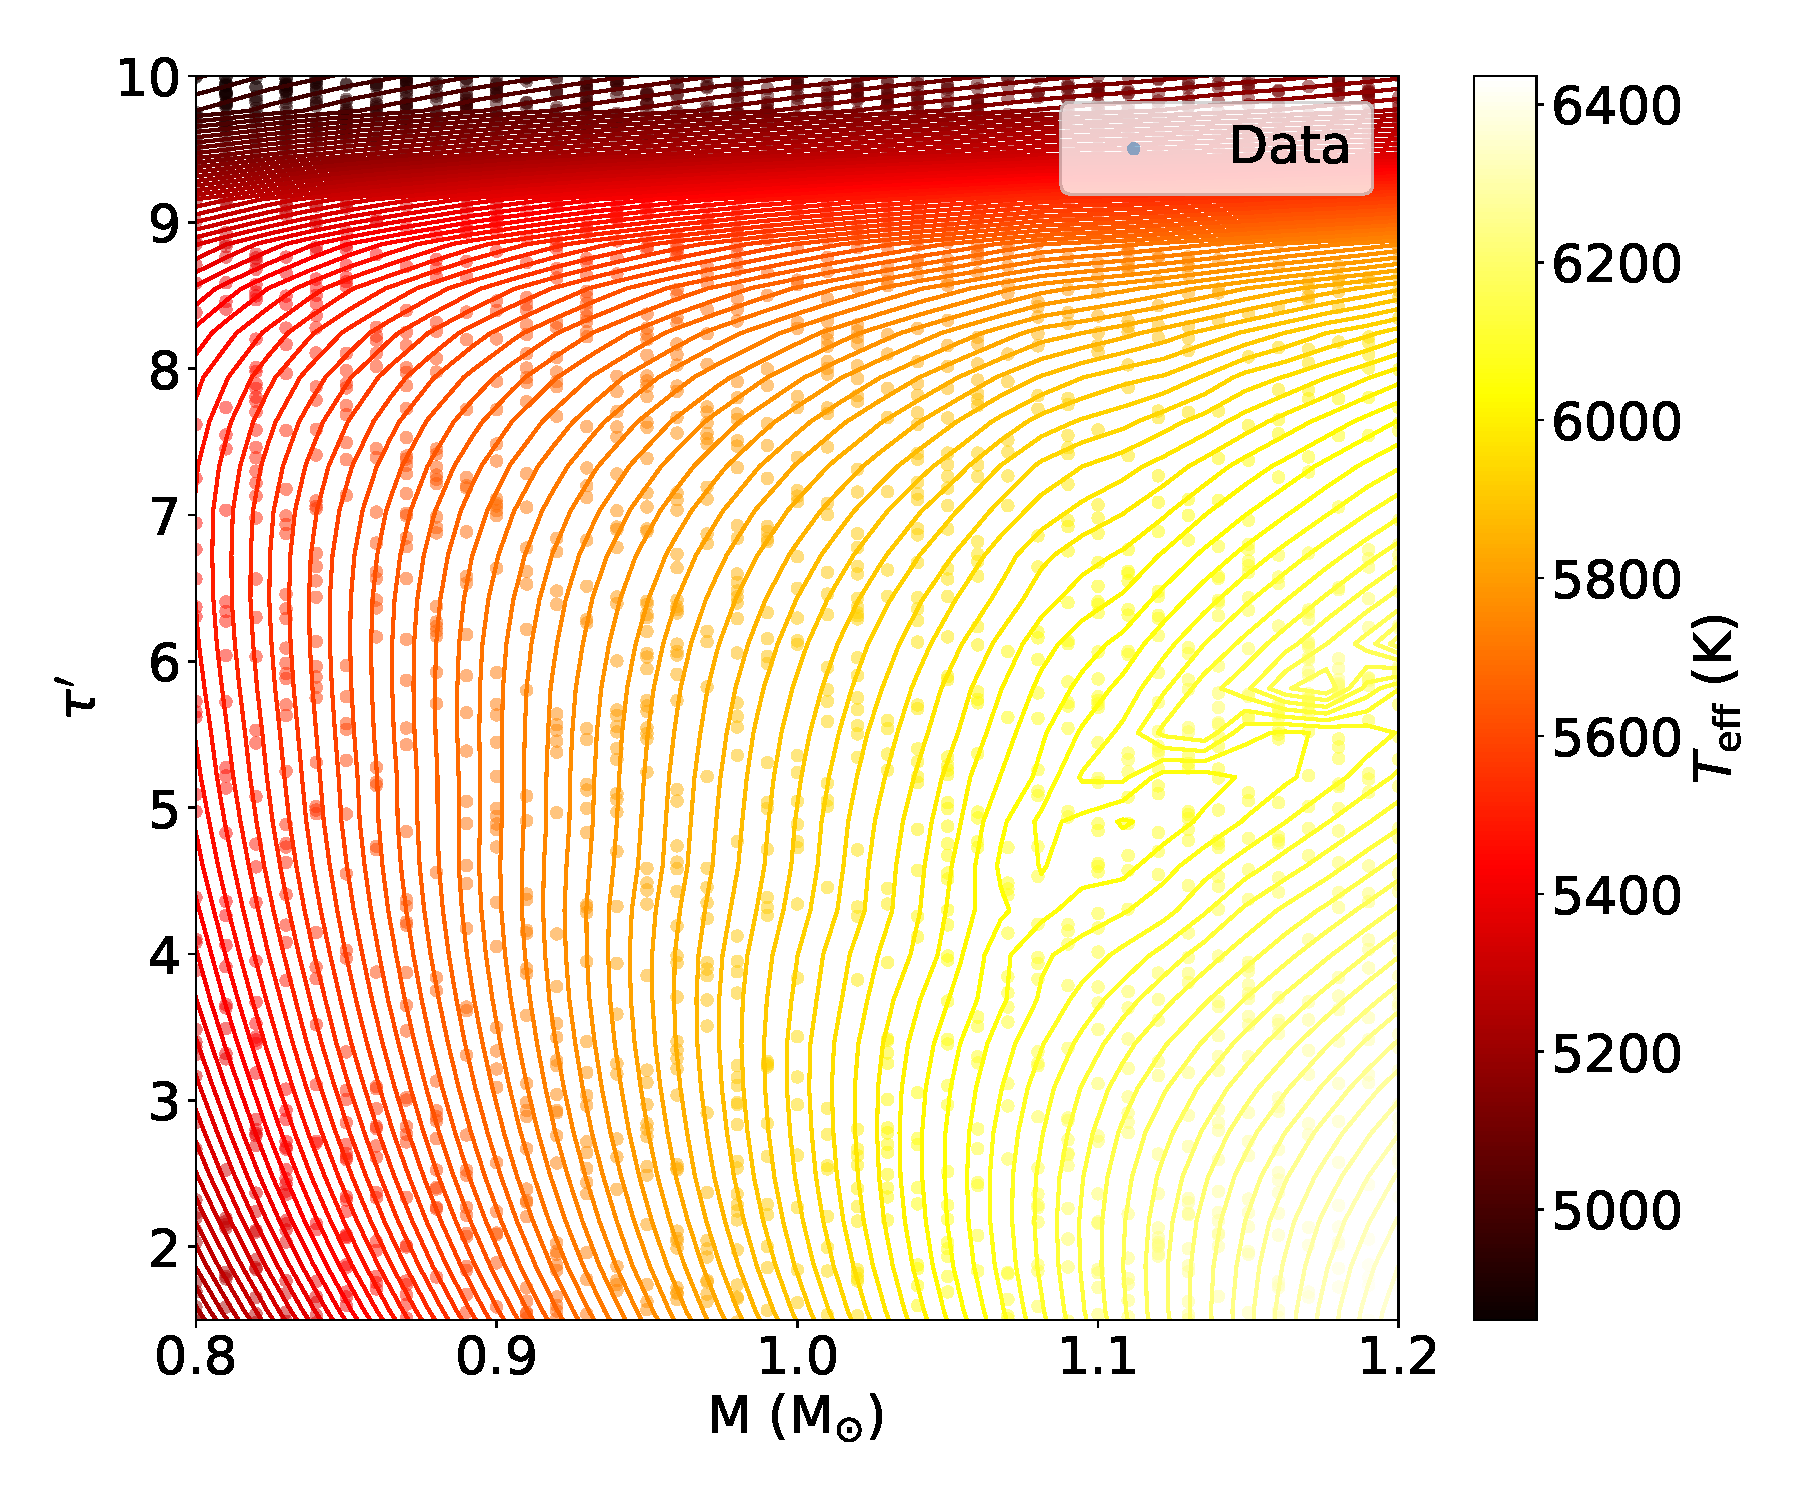
\includegraphics[width=1.0\columnwidth]{2d_gpmodel_MLP.pdf}
    \caption{Top: The GPR model (using the MLP kernel) for the effective temperature ($T_{\rm eff}$) as a function of mass ($M$) and age index ($t'$). Dots represent the training data and counters indicate the GPR predictions. }  
    \label{fig:gpmodel}
\end{figure}


\begin{figure*}
	% To include a figure from a file named example.*
	% Allowable file formats are eps or ps if compiling using latex
	% or pdf, png, jpg if compiling using pdflatex
	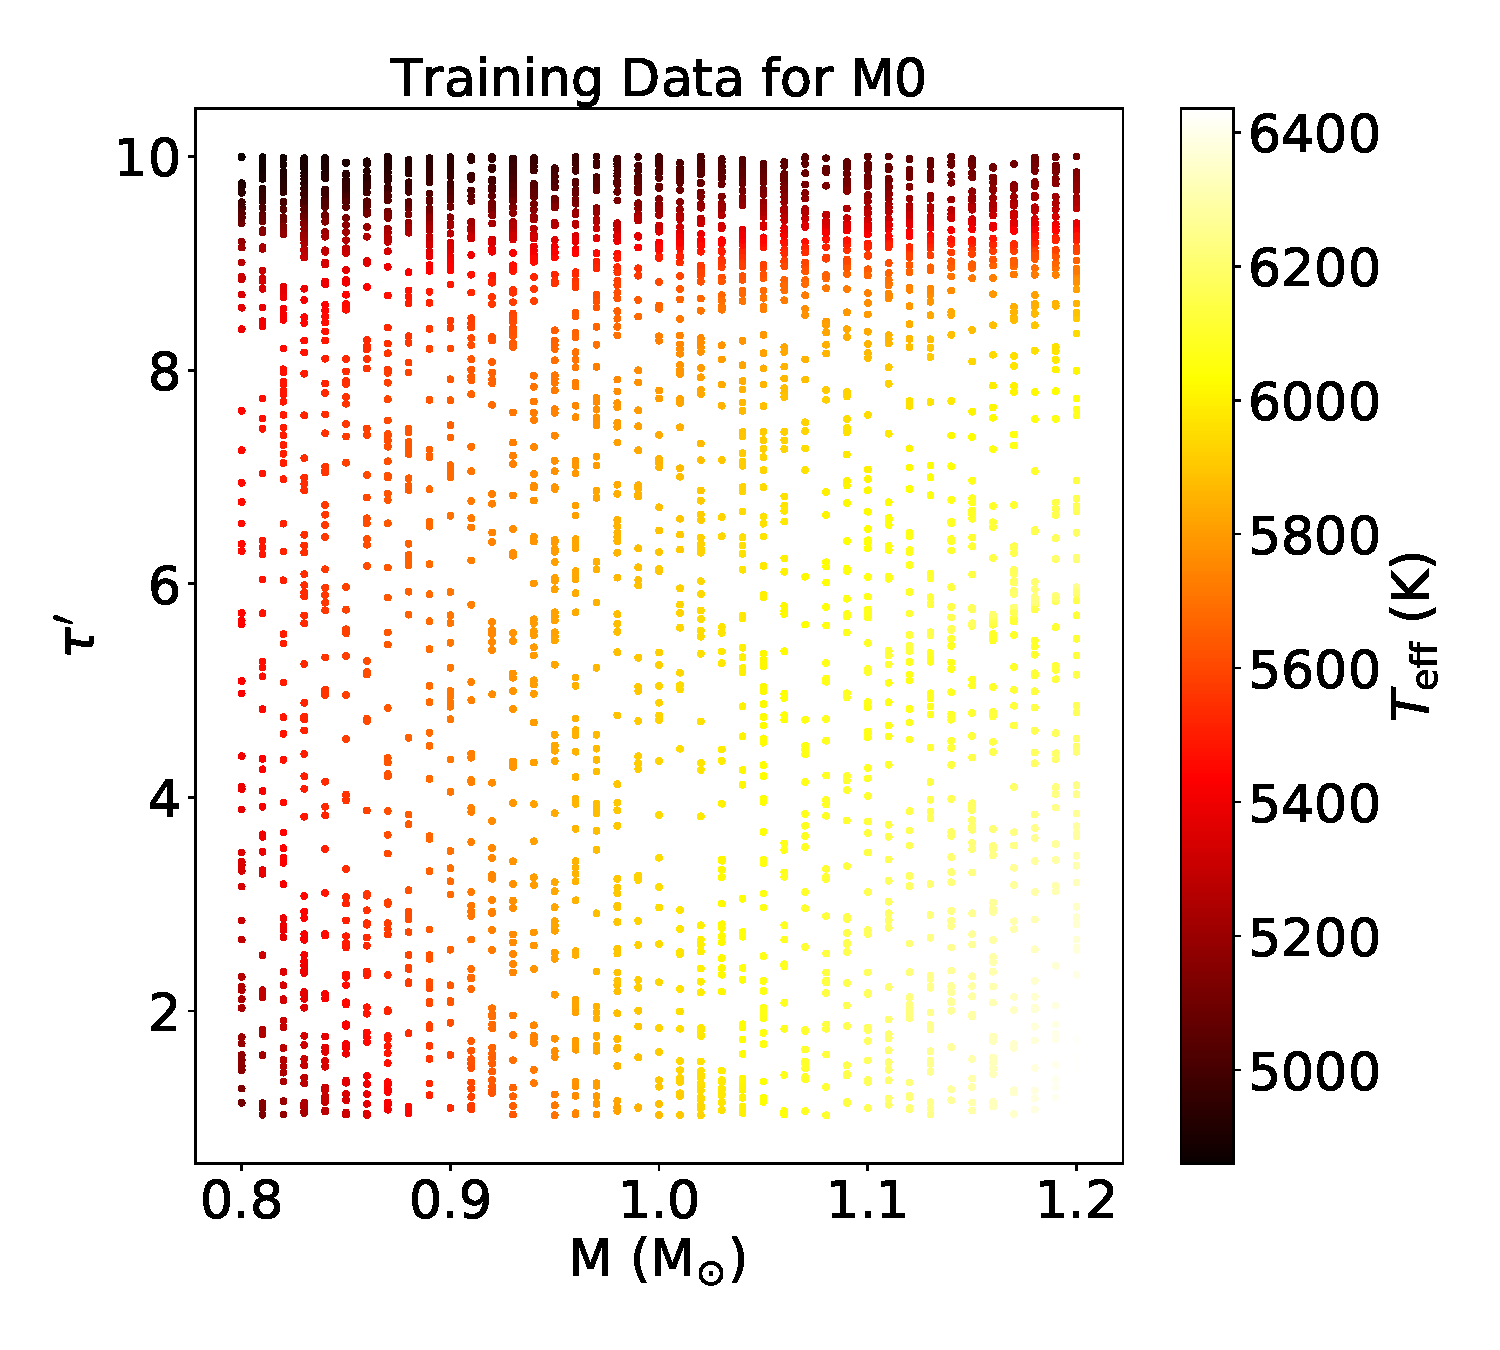
\includegraphics[width=0.33\textwidth]{M0_data.pdf}	
	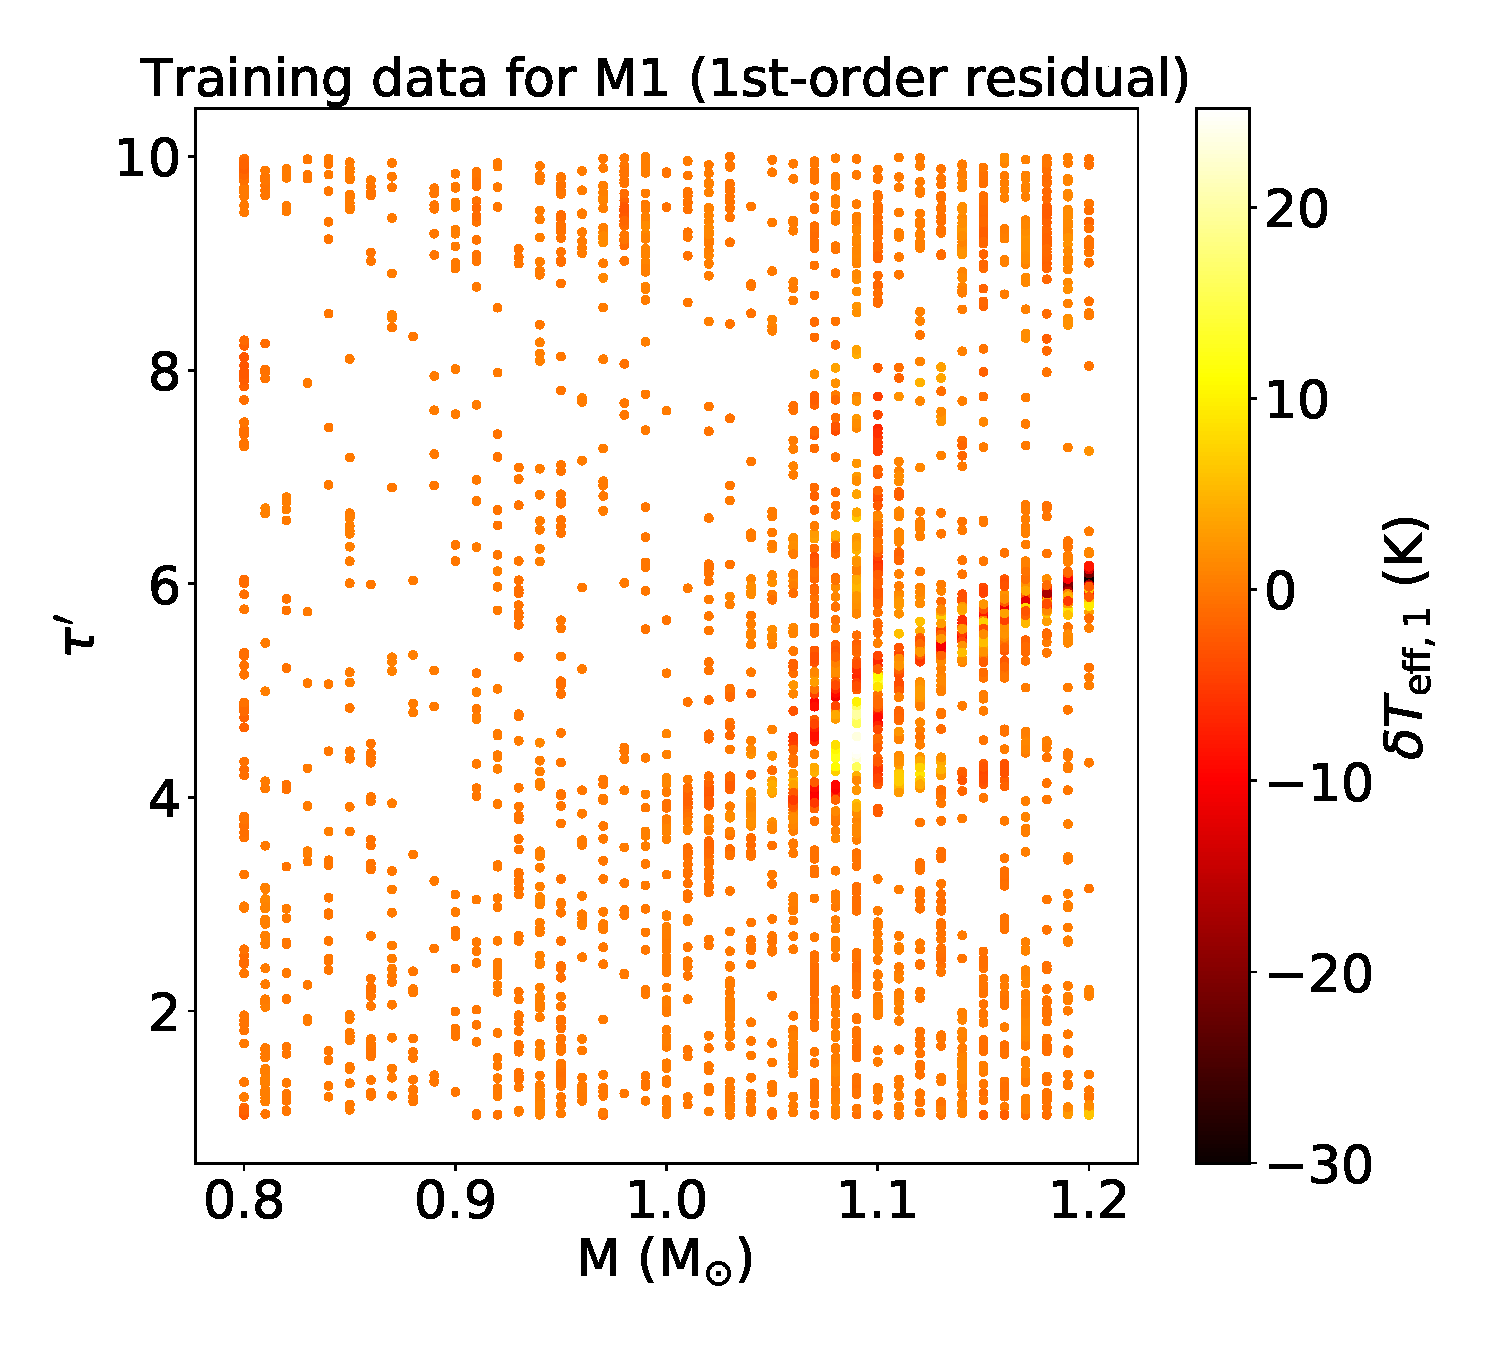
\includegraphics[width=0.33\textwidth]{M1_data.pdf}
	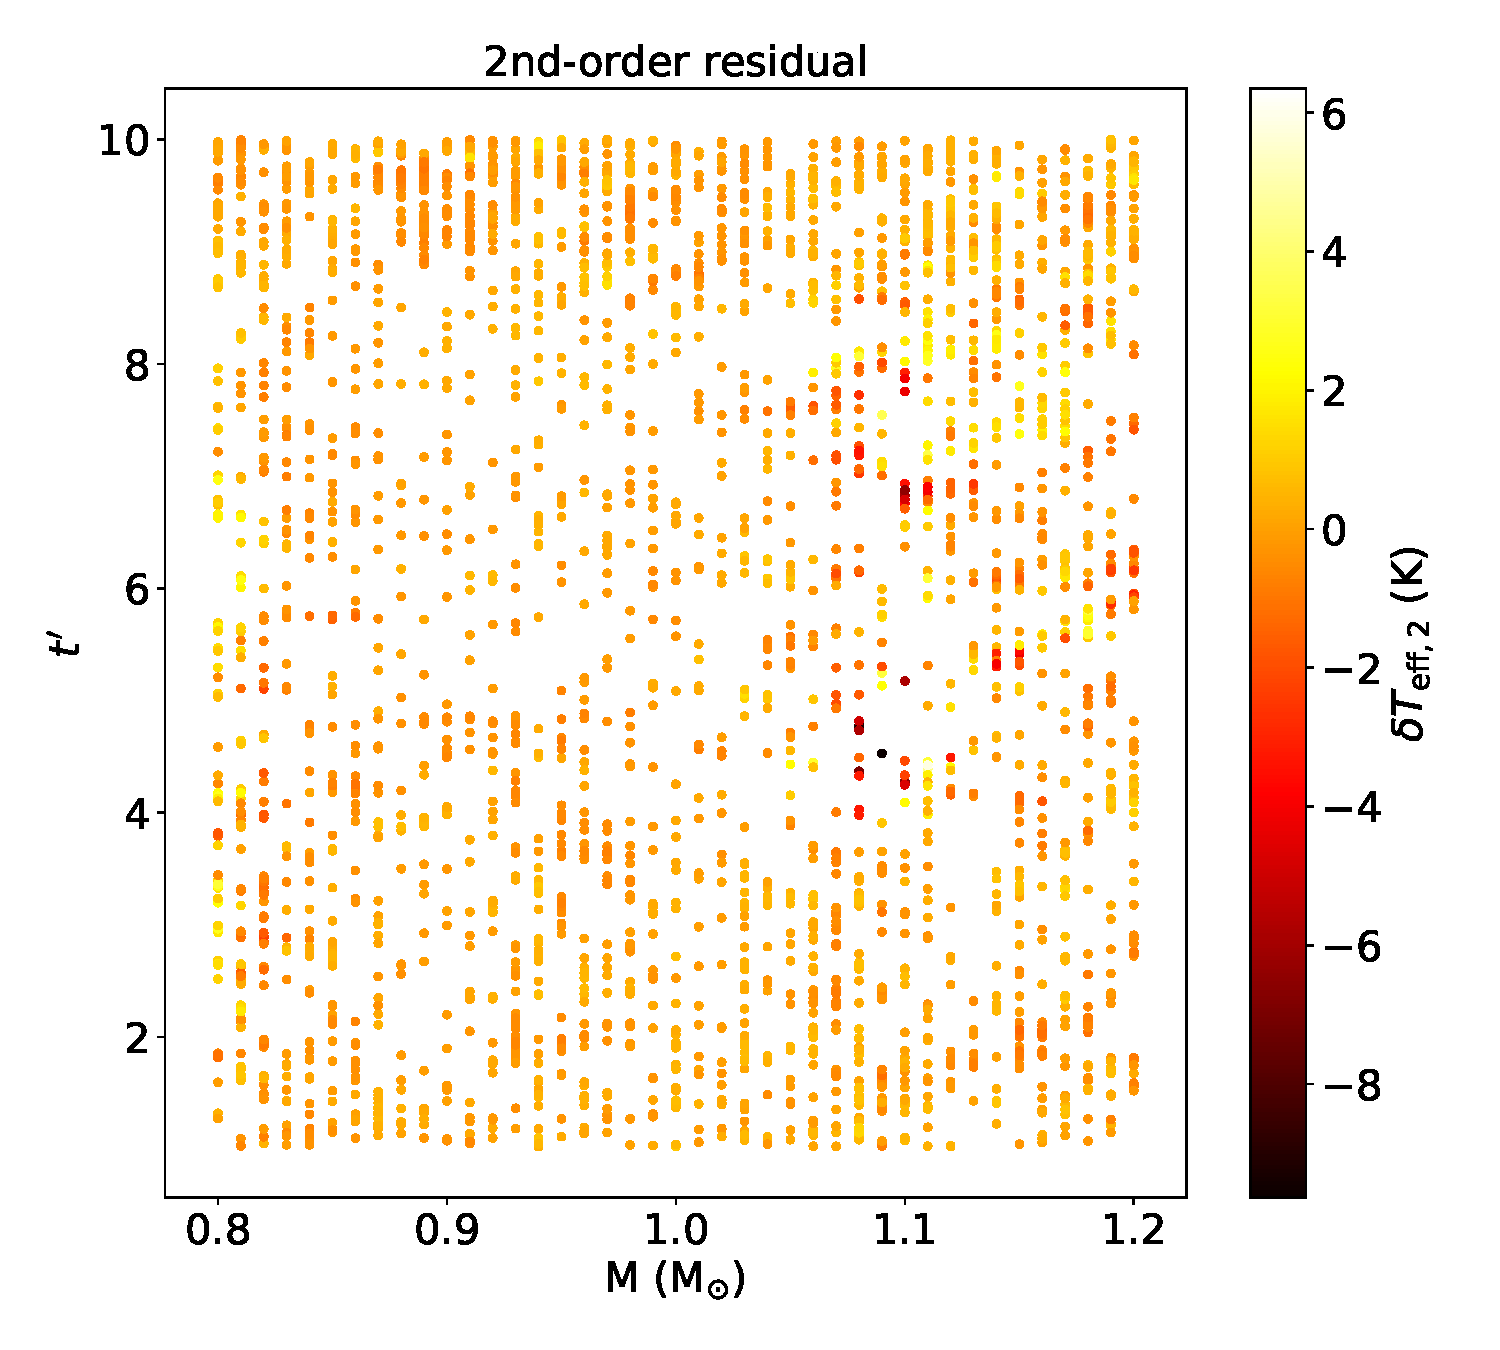
\includegraphics[width=0.33\textwidth]{M2_data.pdf}
		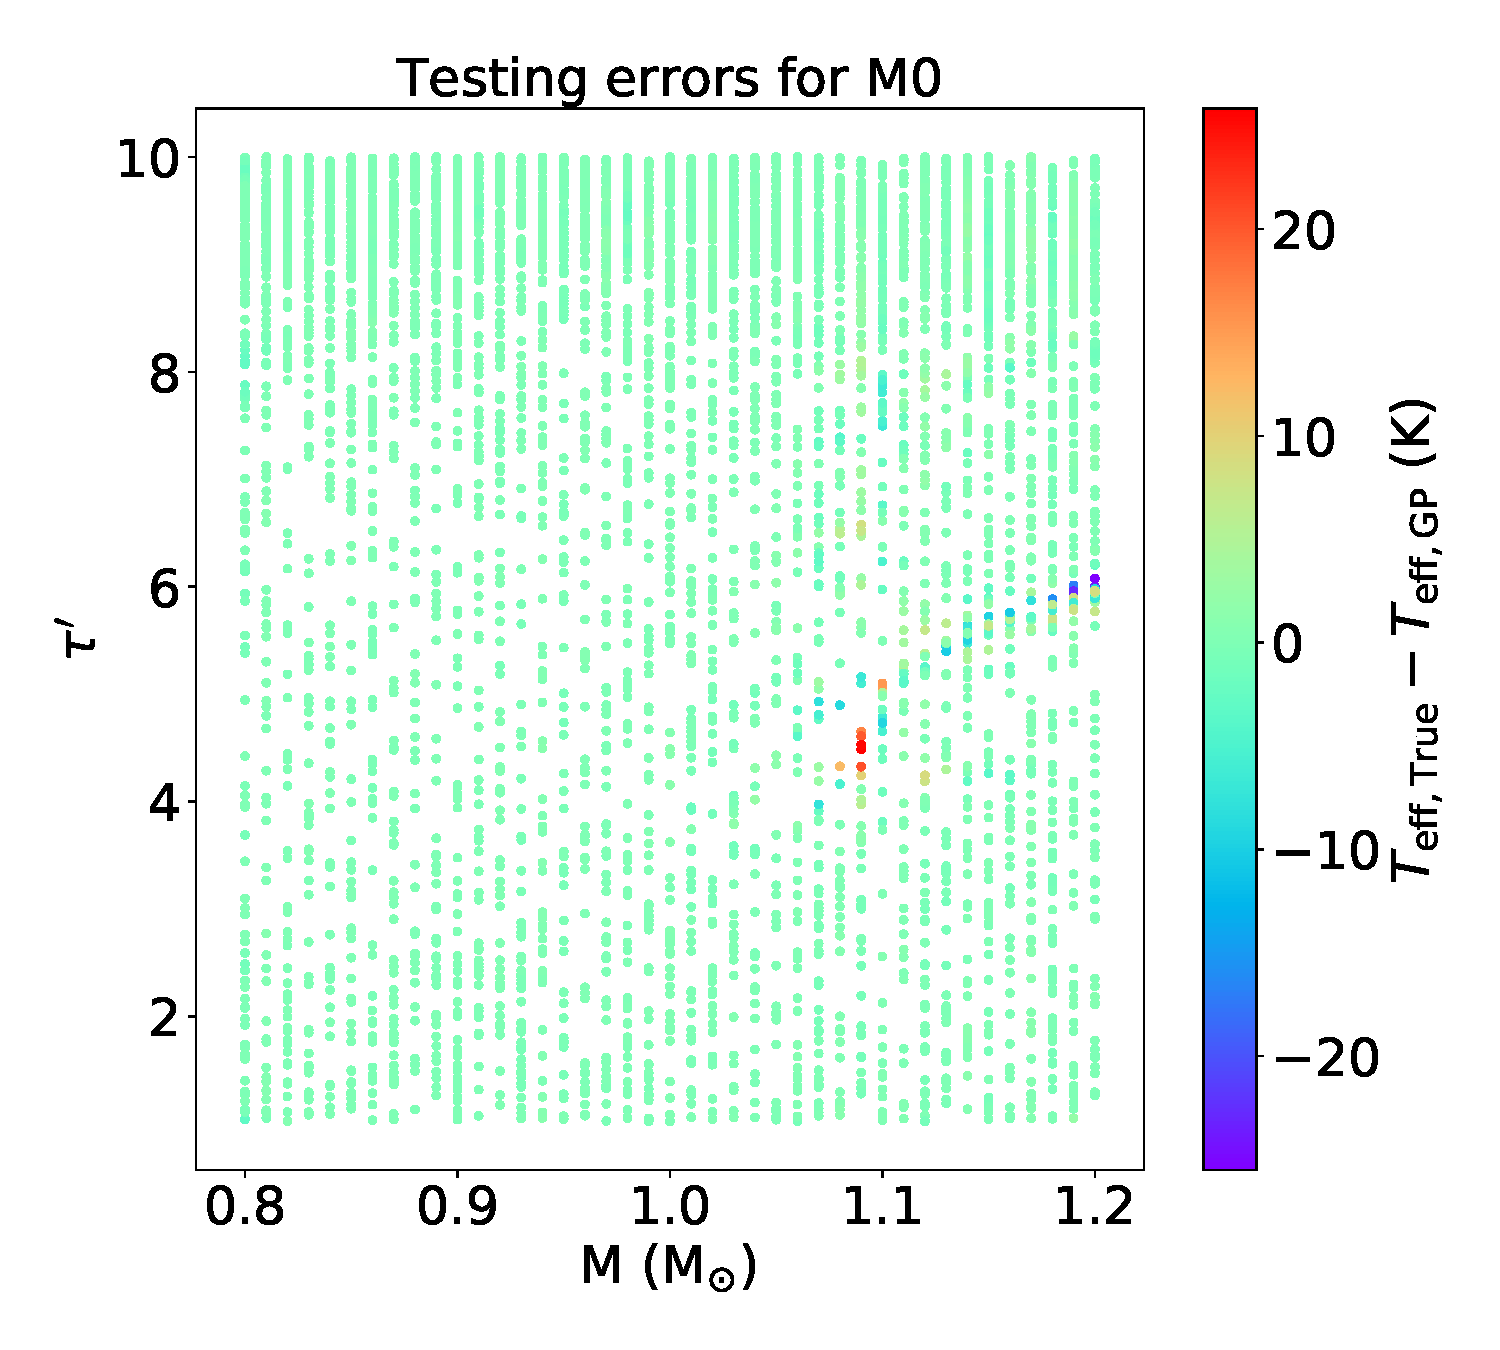
\includegraphics[width=0.33\textwidth]{M0_test.pdf}	
	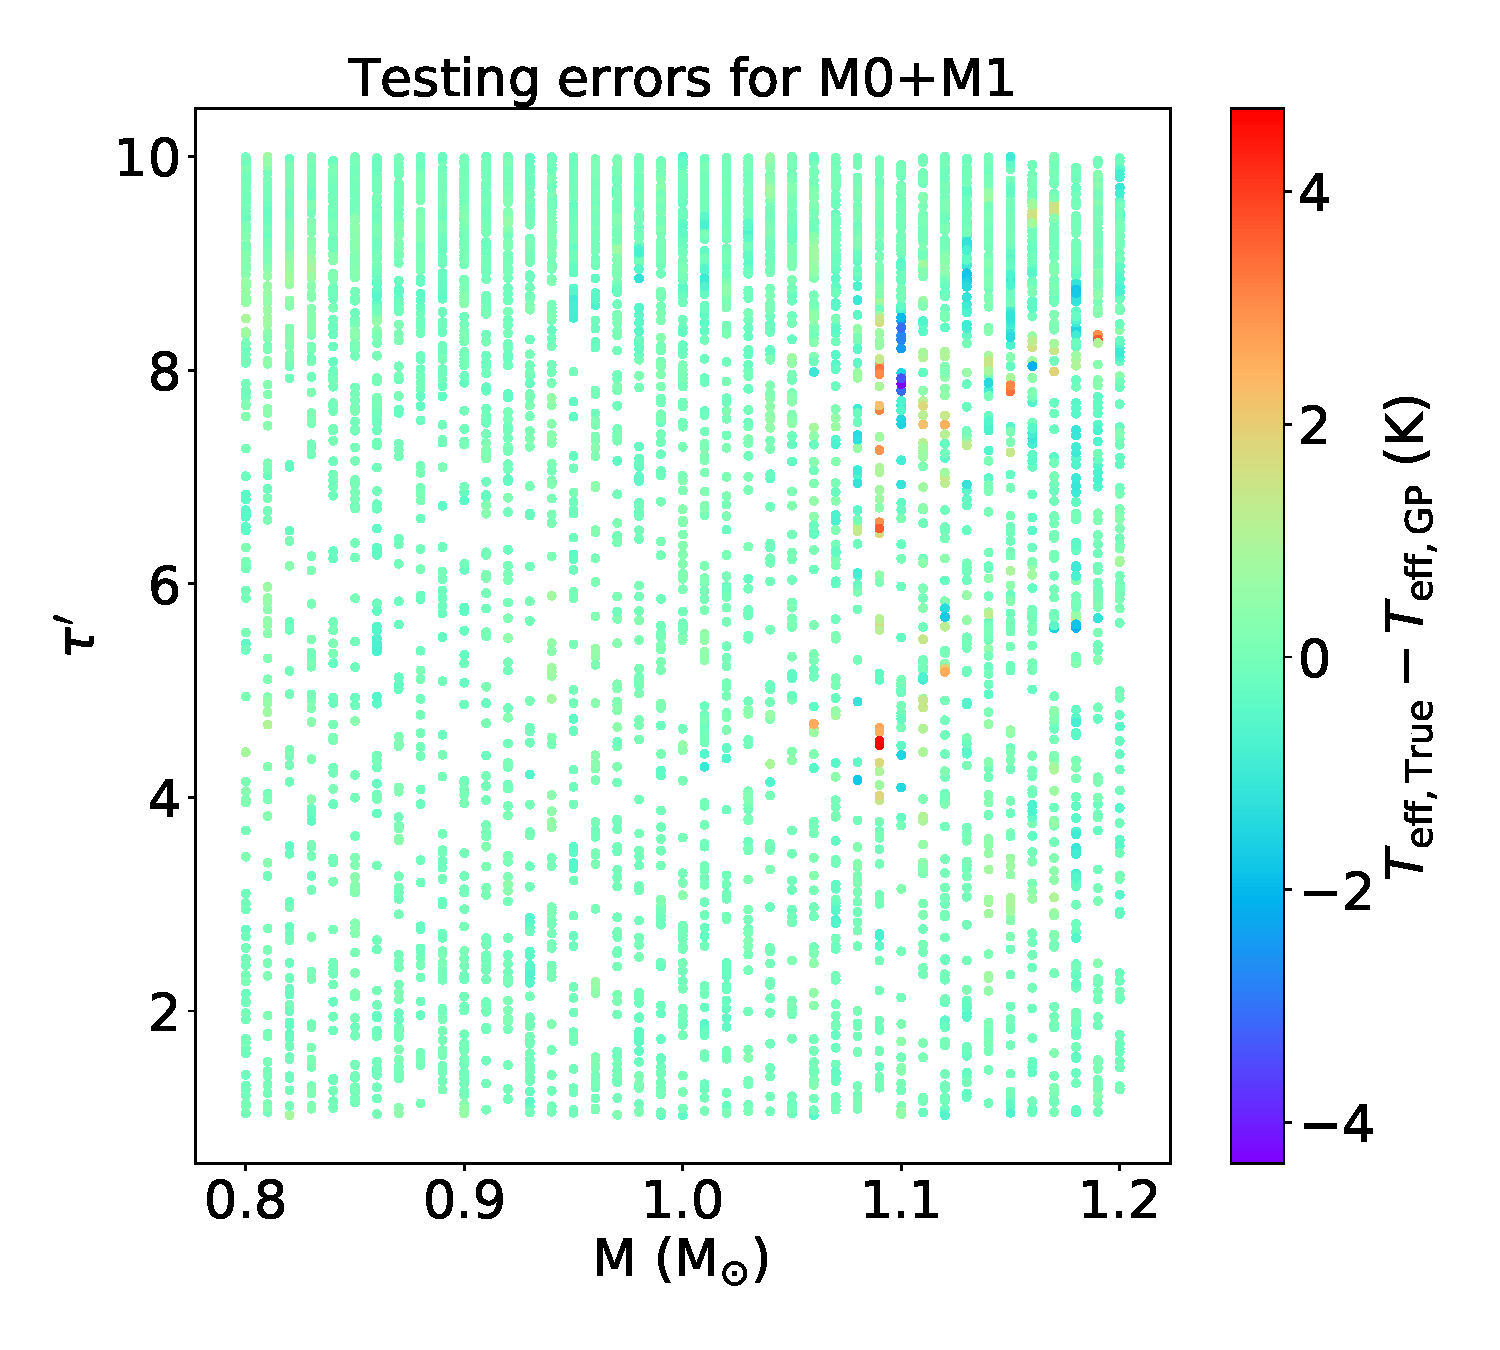
\includegraphics[width=0.33\textwidth]{M1_test.pdf}
	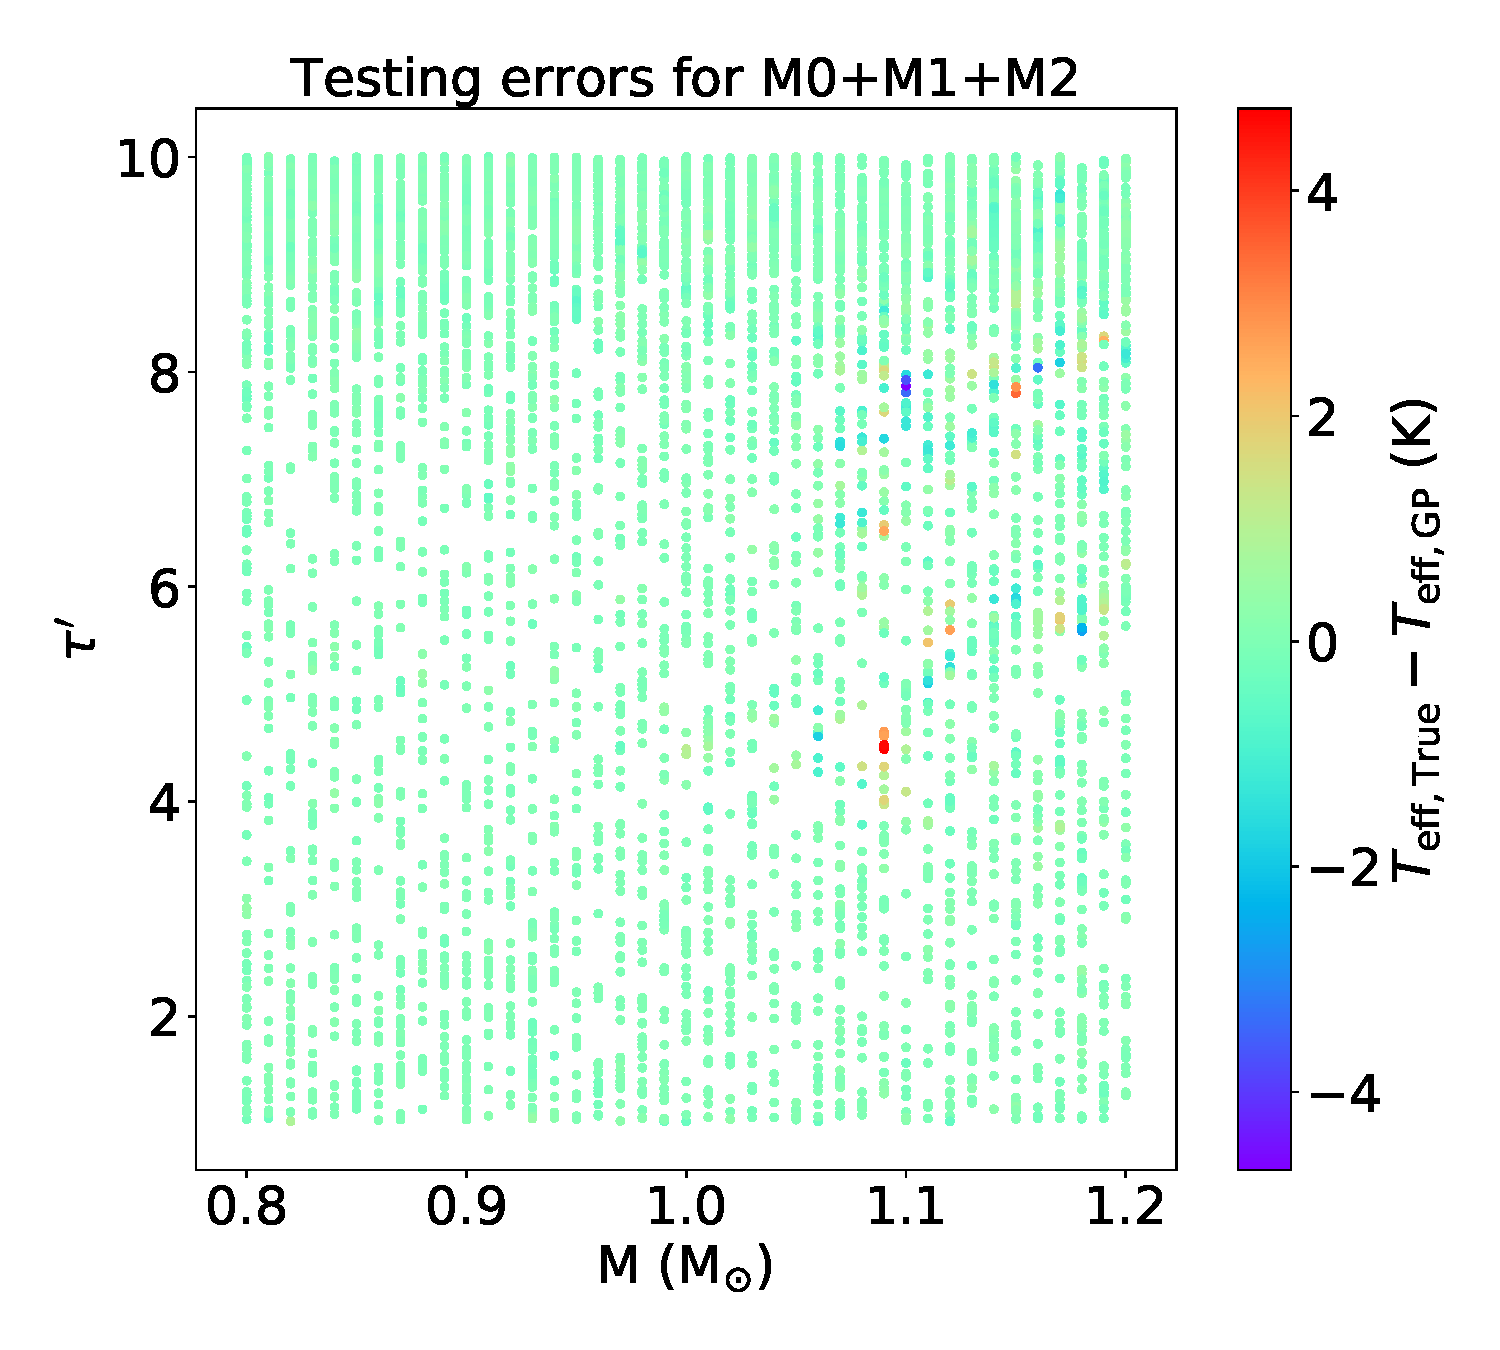
\includegraphics[width=0.33\textwidth]{M2_test.pdf}
    \caption{The data-residual process for training the 2-demission GPR models for the effective temperature. The top row (from left to right) shows the training data used to train the data (M0), the first-order residuals(M1), and the second-order residuals(M2). The bottom row (from left to right) demonstrates the reduction of testing errors along the training process.}  
    \label{fig:drprocess}
\end{figure*}

% \begin{figure}
	% To include a figure from a file named example.*
	% Allowable file formats are eps or ps if compiling using latex
	% or pdf, png, jpg if compiling using pdflatex
%	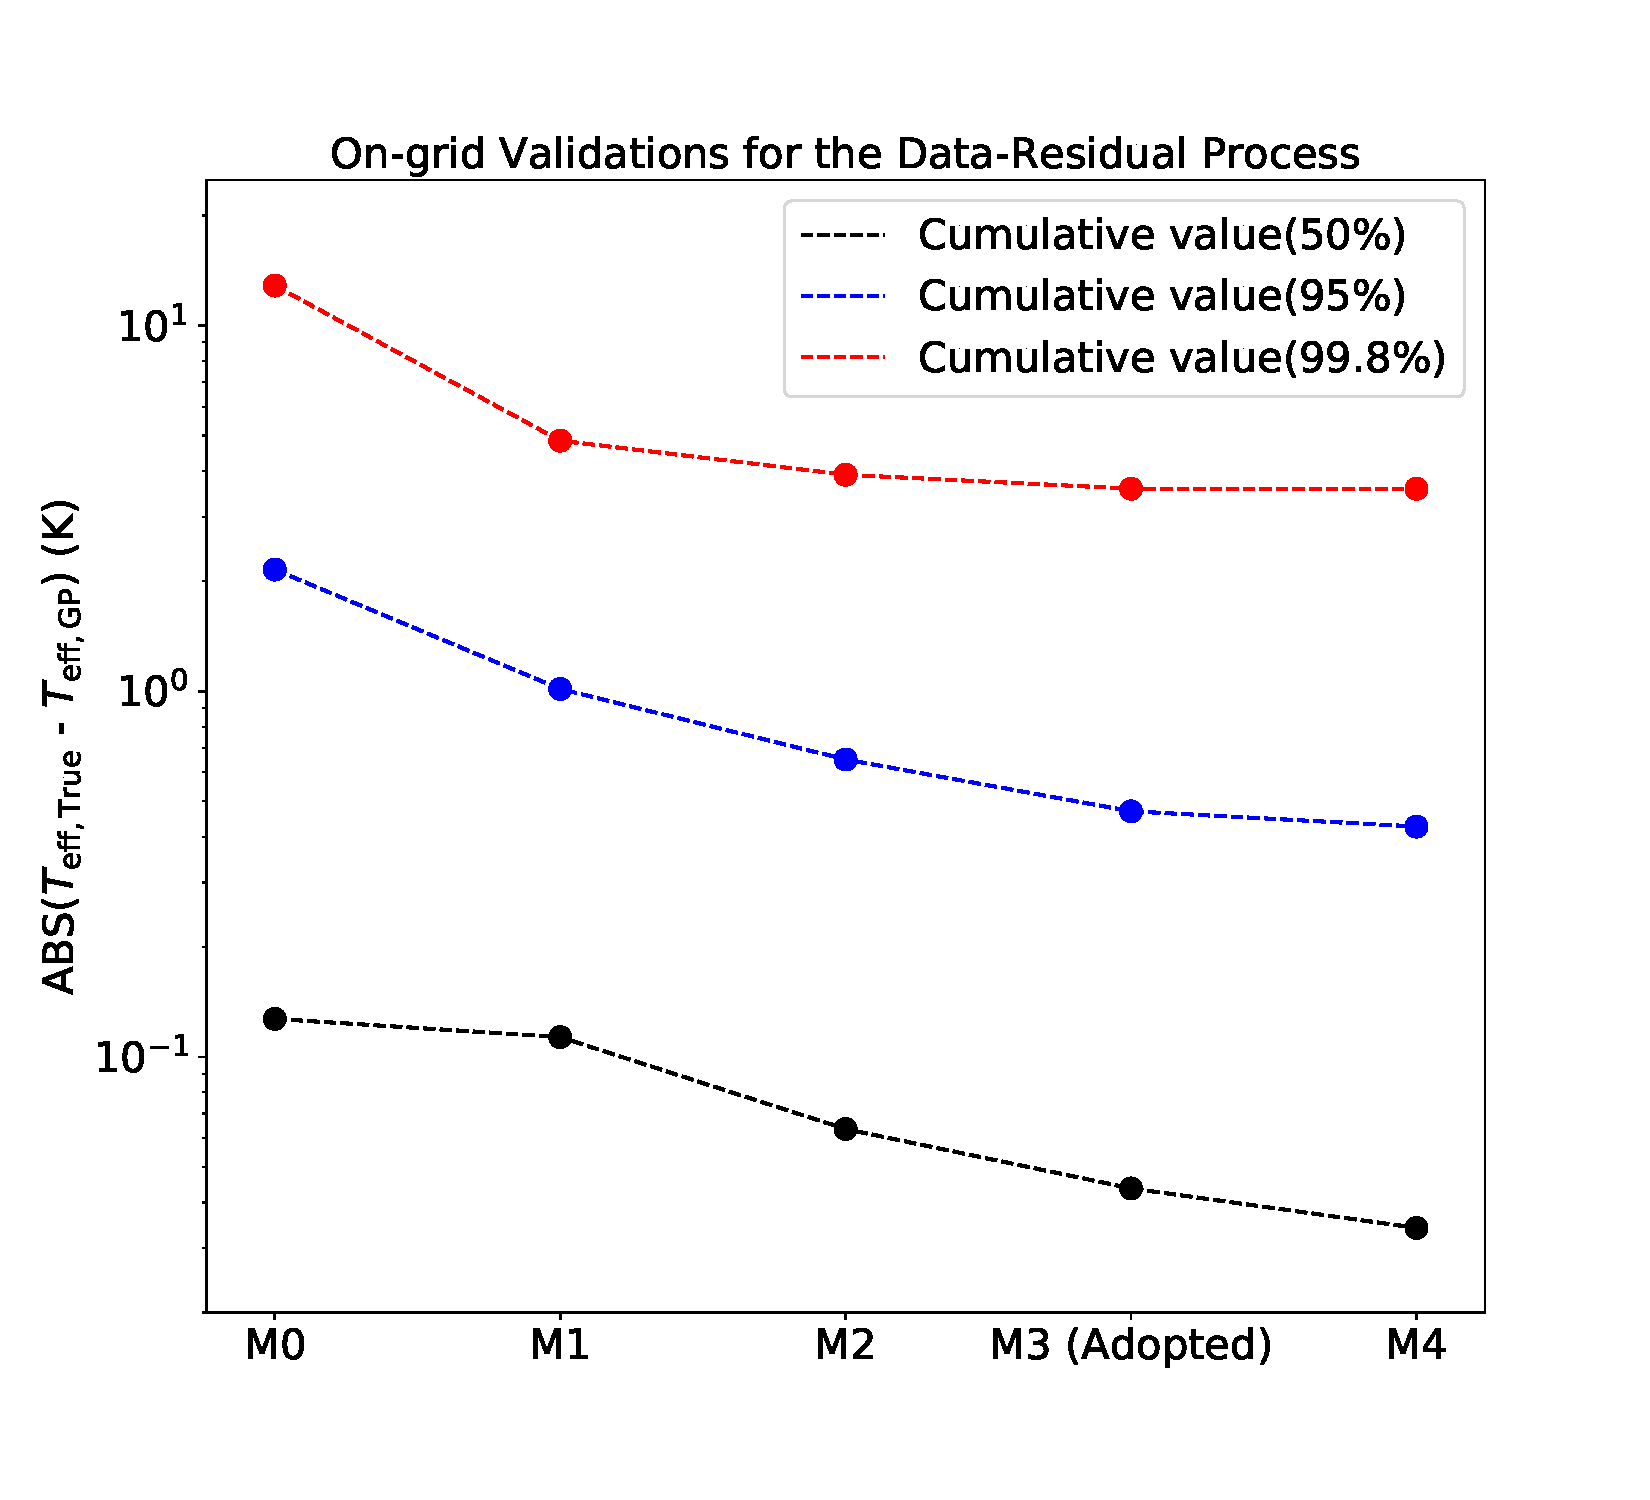
\includegraphics[width=1.0\columnwidth]{all_validations.pdf}
%    \caption{On-grid validations.}  
%    \label{fig:on-grid_validation}
%\end{figure}

\subsubsection{Step 3: Model Validation}

We lastly validated the GPR models by using the offsets between GPR predictions and the validation data (validation errors here after).  We quantified absolute validation errors with three cumulative values at 50\%, 95\%, and 99.8\%. The first two are used to validate GPR models in general level. The last value is used to validate those evolutionary phases where GPR models do not work well. Because a large deviation between the 95\% and 99.8\% cumulative values often means a long tail of probability distribution, which indicates that GPR models poorly describe some local areas. In Figure~\ref{fig:off-grid_validation}, we demonstrated the validation errors for the model combination obtained above. As It can be seen that, the GPR models well predict $T_{\rm eff}$ in most area, however, not very well match those around M$\sim1.1M_{\odot}$ and $\tau'\sim5$ (the main-sequence the hook). Comparing with the testing errors in Figure \ref{fig:drprocess}, the validation errors indicate that although the GPR models were well trained to describe the model grid in this area, they still do not learn the feature between the grid. The reason is that $\sim1.1M_{\odot}$ the boundary between tracks with and without the 'hook'. The local structure is hence more complex than any other areas (as it can be seen in Figure \ref{fig:gpmodel}) and it leads to relatively poor predictions. Because the distribution of validation errors in the input space is not flat, it is difficult to measure a global systematical uncertainty. We will discuss how we applied systematical uncertainty when fitting stars in Section \ref{sec:augmentation}. 
 
 
 \begin{figure}
	% To include a figure from a file named example.*
	% Allowable file formats are eps or ps if compiling using latex
	% or pdf, png, jpg if compiling using pdflatex
	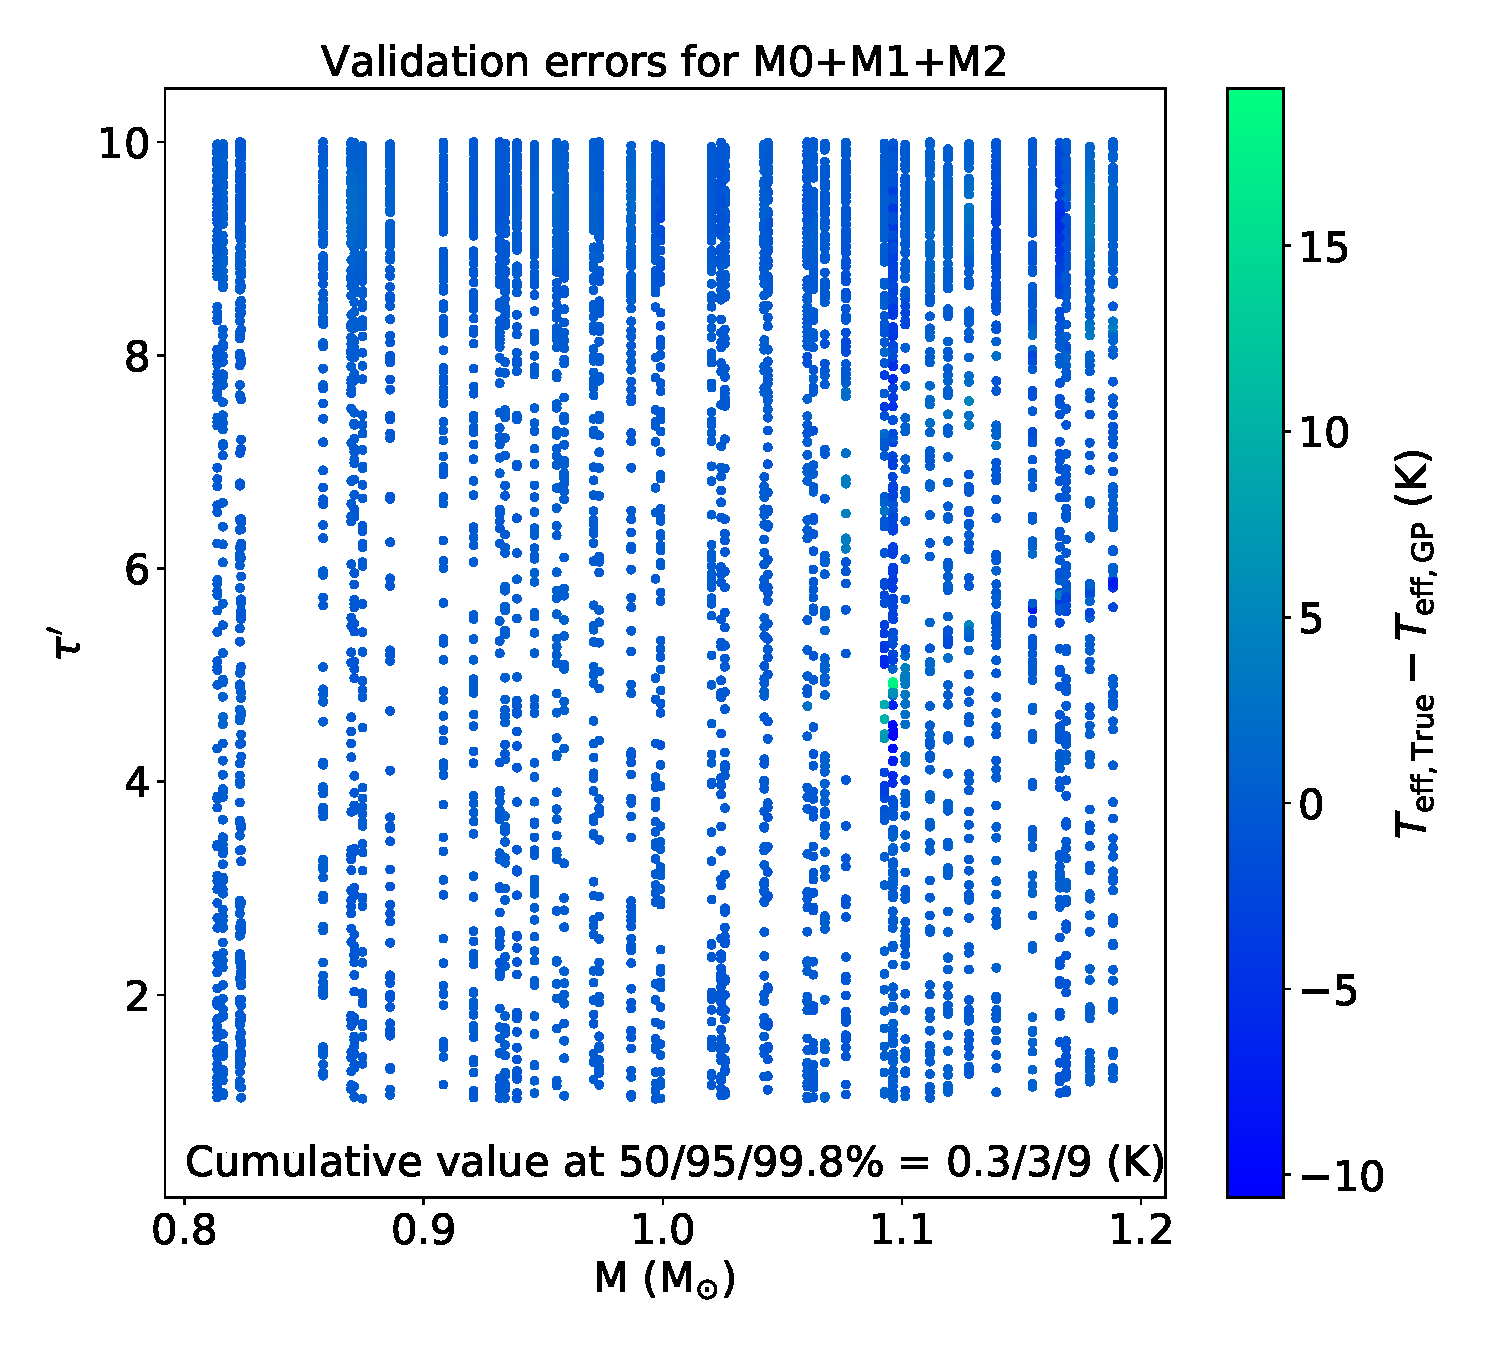
\includegraphics[width=1.0\columnwidth]{off_validation.pdf}
    \caption{Validation errors of $T_{\rm eff}$ on the $M-\tau'$ diagram for the 2-demission GPR models ($T_{\rm eff} = f(M, \tau')$).}  
    \label{fig:off-grid_validation}
\end{figure}

\subsubsection{Summary of the Training Procedure}
Here we summarised our training procedure. We firstly selected three types of data for training, testing, and validating GPR models. The sampling method of training data are different for the outputs depending on their evolving features. The test and validation data were sampled uniformly on the HR diagram to equally cover all evolutionary stages. We then trained GPR models with given inputs and outputs following a data-residual process. A primary model is trained to describe the general feature of the grid, and some extra models are then trained to reveal local structures. A combination of these GPR models is used to describe the \textsc{MESA} grid. Model validation is lastly carried out to validate GPR models and also to estimate systematical uncertainties. With the training process, we trained 2-demission GPR models for $T_{\rm eff}$ and $\log g$, and used them to make a non-sparse $T_{\rm eff}$ - $\log g $ diagram as shown in Figure \ref{fig:gphrdl}. 
 
\begin{figure}
	% To include a figure from a file named example.*
	% Allowable file formats are eps or ps if compiling using latex
	% or pdf, png, jpg if compiling using pdflatex
	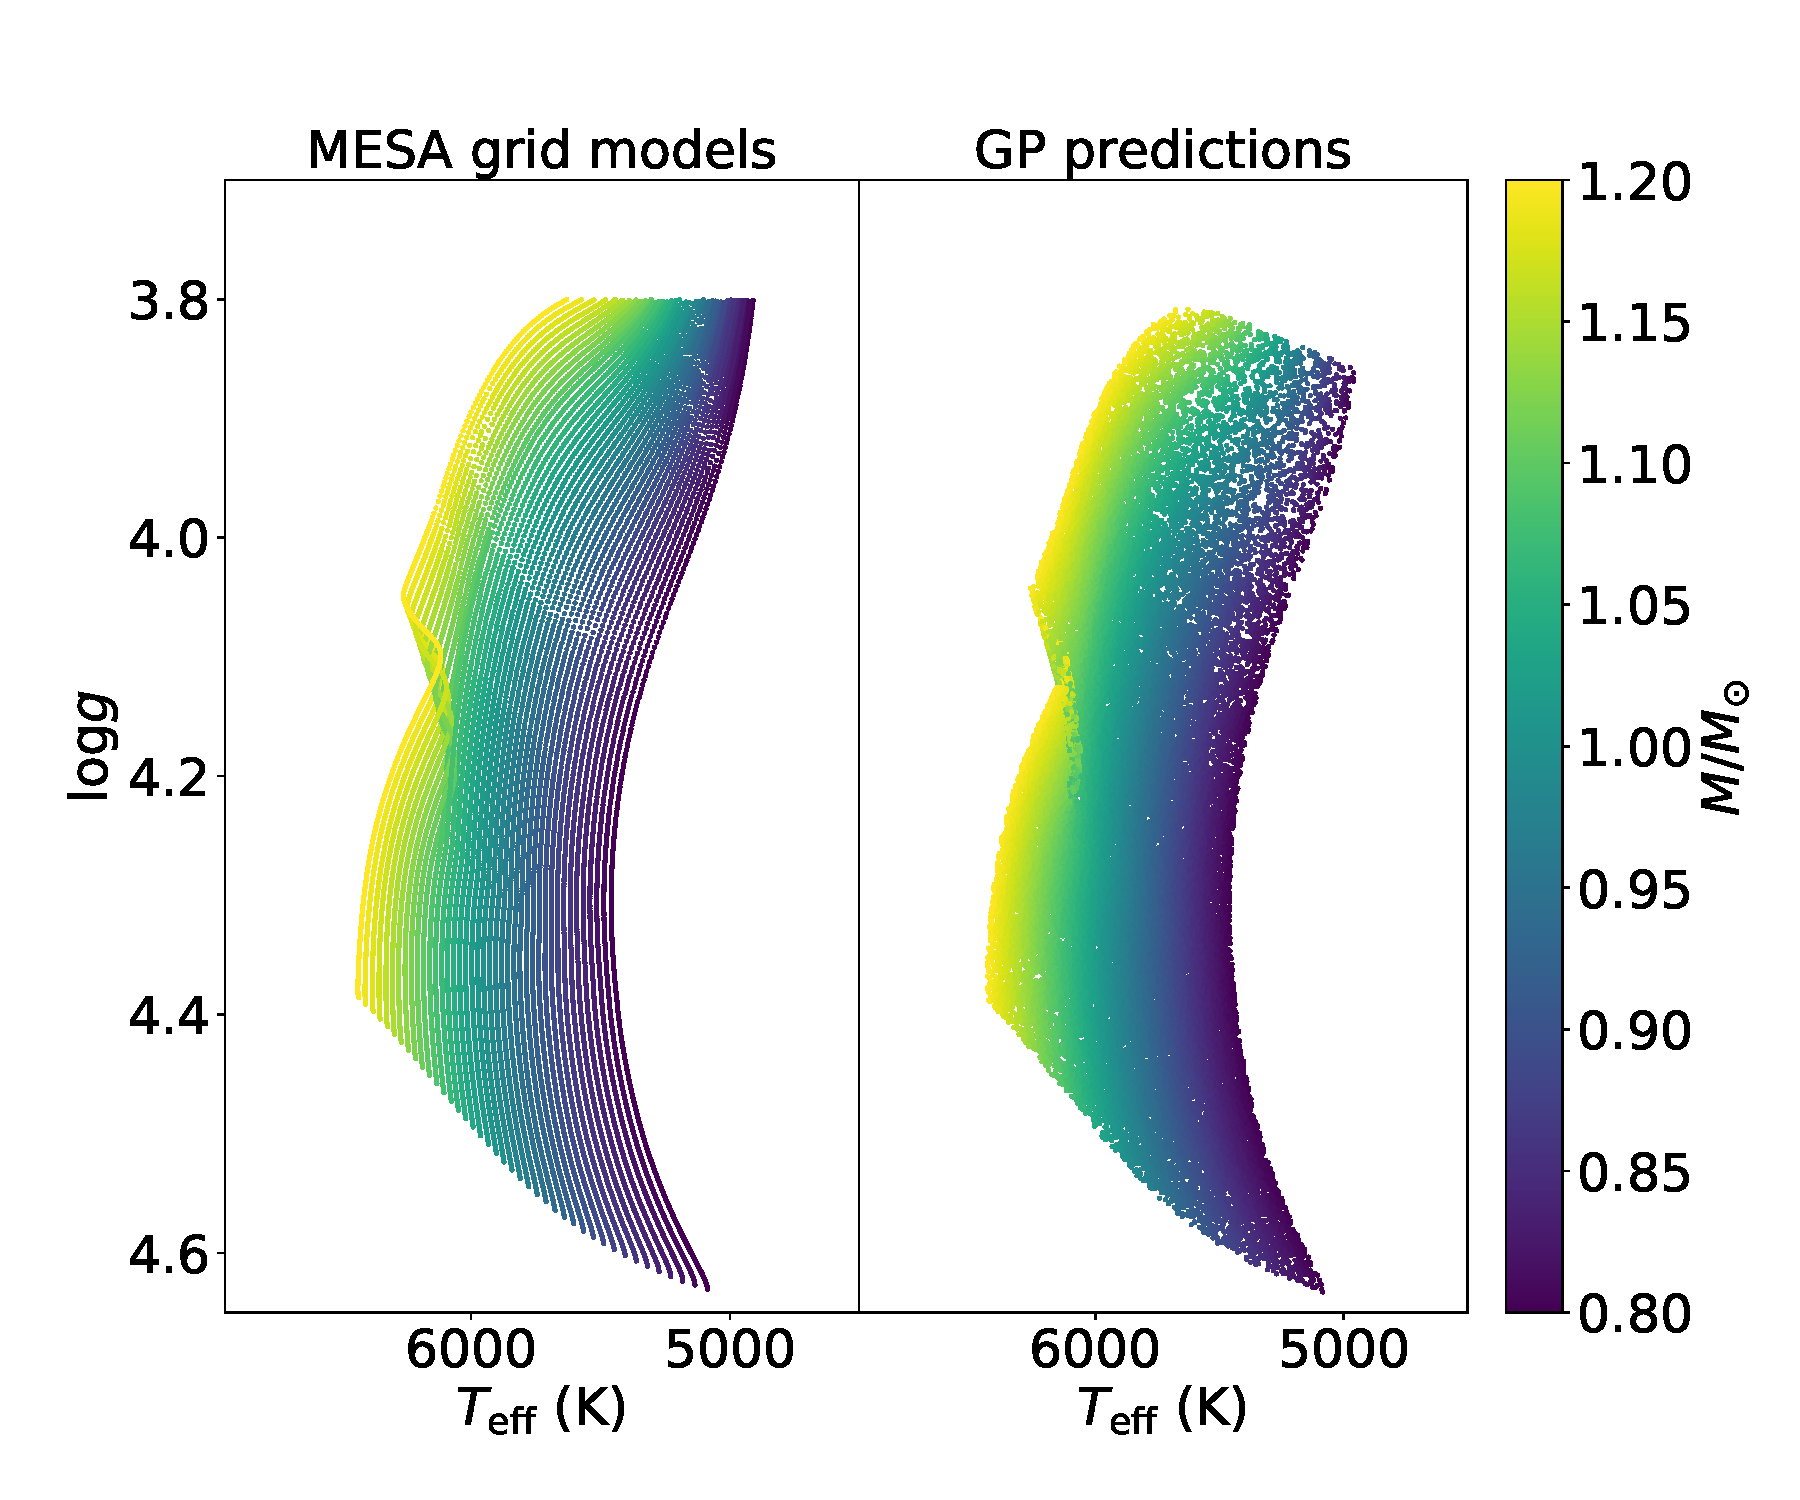
\includegraphics[width=1.0\columnwidth]{2d_hrd_compare.pdf}
    \caption{MESA grid models (sparse) and GP predictions (non-sparse) on the $T_{\rm eff}$ - $\log g$ diagram. Note that we only predict models with $\log$ >= 3.8 to avoid the edge effect. }
    \label{fig:gphrdl}
\end{figure}


